\documentclass[11pt,a4paper]{article}

\usepackage[utf8]{inputenc}
\usepackage[T1]{fontenc}
\usepackage[margin=2.0cm]{geometry}
\usepackage{amsmath,amssymb,amsthm}
\usepackage{booktabs}
\usepackage{longtable}
\usepackage{graphicx}
\usepackage{hyperref}
\usepackage{fancyhdr}
\usepackage{xcolor}
\usepackage{enumitem}

\hypersetup{
    colorlinks=true,
    linkcolor=teal!70!black,
    urlcolor=blue!70!black,
    citecolor=teal!70!black
}

\pagestyle{fancy}
\fancyhf{}
\lhead{\small CSC14003 $|$ Introduction to Artificial Intelligence}
\rhead{\small Project 2: No-Guess Griductive Solver}
\lfoot{\small Faculty of Information Technology, University of Science, VNU-HCM}
\rfoot{\small Page \thepage}
\renewcommand{\headrulewidth}{0.4pt}
\renewcommand{\footrulewidth}{0.4pt}

\newtheorem{theorem}{Theorem}[section]
\newtheorem{proposition}[theorem]{Proposition}

\title{\textbf{\LARGE Project 2: No-Guess Griductive Solver}\\[4pt]
\large Propositional Logic, Automatic CNF Encoding, and Custom DPLL SAT Deduction}
\author{Faculty of Information Technology, University of Science, VNU-HCM\\
\textbf{Demonstration Video (Google Drive):} \url{https://drive.google.com/drive/folders/REPLACE_WITH_YOUR_PUBLIC_DRIVE_LINK}}
\date{}

\begin{document}
\maketitle
\thispagestyle{fancy}

\section{Project Planning and Task Distribution}
The project was executed over a structured three-week engineering schedule divided into four strictly decoupled subsystems: (1) Logical Representation, Region Resolution, and Direct Semantic Evaluation; (2) Automatic CNF Encoding and Custom Pure-Python DPLL SAT Solver; (3) No-Guess Deductive Agent, Witness-Guided Pruning, Uniqueness Checking, and Deletion-Based MUS Hinting; and (4) Interactive Web GUI, Coupled Backtracking Benchmark Suite, and Experimental Analysis. Individual grades follow $\text{Individual Score} = \text{Group Score} \times \text{Completion \%}$.

\begin{table}[h!]
\centering
\small
\begin{tabular}{@{}llp{8.4cm}c@{}}
\toprule
\textbf{Student ID} & \textbf{Full Name} & \textbf{Assigned Responsibilities \& Deliverables} & \textbf{Completion} \\
\midrule
\texttt{StudentID\_1} & Member 1 Full Name & Core board/clue data models, 4 core regions + Extension 1 advanced regions, \texttt{ClueValidator}, standalone \texttt{SemanticEvaluator} & 100\% \\
\texttt{StudentID\_2} & Member 2 Full Name & Automatic \texttt{CNFEncoder} (Combinatorial, Sinz Sequential Counter, Extensions 2--5), custom \texttt{DPLLSolver} \& branching heuristics & 100\% \\
\texttt{StudentID\_3} & Member 3 Full Name & \texttt{GameEngine}/\texttt{LogicAgent} isolation, witness-guided deduction loop, \texttt{UniquenessChecker}, deletion-based MUS \texttt{HintEngine} & 100\% \\
\texttt{StudentID\_4} & Member 4 Full Name & Interactive GUI + live CNF Inspector, 19-puzzle suite (including coupled stress cases), automated benchmarks, charts, report \& video & 100\% \\
\bottomrule
\end{tabular}
\caption{Team responsibilities and task completion percentages.}
\end{table}

\section{Problem Formulation and System Architecture}

\subsection{Propositional Variables and Deterministic Mapping}
An $N \times N$ Griductive board ($N \in \{3, 4, 5\}$) indexes rows $r \in \{1, \dots, N\}$ from top to bottom and columns $c \in \{0, \dots, N-1\}$ ($\text{A}, \text{B}, \dots$) from left to right. Characters are ordered alphabetically in canonical row-major order $i = (r - 1)N + c + 1 \in \{1, \dots, N^2\}$. For each character $i$, \texttt{VariableManager} assigns one primary Boolean variable:
\[
C_i = \begin{cases}
\text{True}, & \text{if character } i \text{ is a Criminal,} \\
\text{False}, & \text{if character } i \text{ is Innocent.}
\end{cases}
\]
Auxiliary variables required by sequential counters, regional comparisons, Tseitin XOR chains, disjunction selectors, or BFS connectivity layers are allocated strictly in the disjoint integer range $\{N^2 + 1, N^2 + 2, \dots\}$.

\subsection{Core Clue Language and Five Distinct Extension Families}
Every revealed clue is guaranteed \textbf{true} regardless of its owner's status. Let $\llbracket C_i \rrbracket \in \{0, 1\}$ denote the indicator of $C_i = \text{True}$. Beyond the four required regions (\texttt{ROW}, \texttt{COL}, 8-\texttt{NEIGHBORS} excluding self, and explicit \texttt{CELL\_LIST}) and six required core templates, we implement \textbf{five distinct extension families} covering every extension class in Section 3.2 and Figure 1 of the specification:

\begin{table}[h!]
\centering
\small
\begin{tabular}{@{}llp{9.2cm}@{}}
\toprule
\textbf{Category} & \textbf{Template} & \textbf{Formal Logical Semantics} \\
\midrule
Core 1 & \texttt{FACT(i, status)} & Unit literal $C_i$ (Criminal) or $\neg C_i$ (Innocent). \\
Core 2 & \texttt{SAME(i, j)} & Bi-implication $C_i \leftrightarrow C_j$. \\
Core 3 & \texttt{DIFFERENT(i, j)} & Exclusive-OR $C_i \oplus C_j$. \\
Core 4 & \texttt{EXACTLY(k, R)} / \texttt{NO(R)} & $\sum_{i \in R} \llbracket C_i \rrbracket = k$ (\texttt{NO(R)} is normalized to $k = 0$). \\
Core 5 & \texttt{AT\_LEAST(k, R)} & $\sum_{i \in R} \llbracket C_i \rrbracket \ge k$, where $0 \le k \le |R|$. \\
Core 6 & \texttt{AT\_MOST(k, R)} & $\sum_{i \in R} \llbracket C_i \rrbracket \le k$, where $0 \le k \le |R|$. \\
\midrule
Extension 1 & \texttt{ADVANCED\_REGIONS} & $R_1 \cap R_2$ (\texttt{INTERSECTION}), \texttt{COMMON\_NEIGHBORS(i,j)}, \texttt{CORNERS}, \texttt{BOUNDARY}, \texttt{BETWEEN(i,j)}, \texttt{DIRECTIONAL(i,dir)}, \texttt{PROFESSION(role)}. \\
Extension 2 & \texttt{COMPARE\_COUNT} & \texttt{MORE\_CRIMINALS}$(R_1, R_2)$: $\sum_{i \in R_1} \llbracket C_i \rrbracket > \sum_{j \in R_2} \llbracket C_i \rrbracket$; \texttt{EQUAL\_CRIMINALS}$(R_1, R_2)$: equality. \\
Extension 3 & \texttt{PARITY(R, ODD|EVEN)} & $\big(\sum_{i \in R} \llbracket C_i \rrbracket\big) \bmod 2 = 1$ (\texttt{ODD}) or $0$ (\texttt{EVEN}). \\
Extension 4 & \texttt{COMPOUND(op, $\Phi_1, \Phi_2$)} & $\Phi_1 \land \Phi_2$ (\texttt{AND}), $\Phi_1 \lor \Phi_2$ (\texttt{OR}), or $\Phi_1 \to \Phi_2$ (\texttt{IMPLIES}). \\
Extension 5 & \texttt{CONNECTED(R, status)} & Active \texttt{status} cells in $R$ induce $\le 1$ 4-connected grid component. \\
\bottomrule
\end{tabular}
\caption{Complete structured clue language (6 required core templates + 5 distinct extensions).}
\end{table}

\subsection{Public Knowledge Base $KB_t$ and Architectural Reveal Protocol}
At step $t$, let $\mathcal{R}_t \subseteq \{1, \dots, N^2\}$ be the set of revealed cards. The public knowledge base is:
\[
KB_t = \left(\bigwedge_{i \in \mathcal{R}_t} \text{CNF}(\text{clue}_i)\right) \land \left(\bigwedge_{i \in \mathcal{R}_t} U(i, \text{status}_i)\right), \quad U(i, \text{Criminal}) = (C_i),\; U(i, \text{Innocent}) = (\neg C_i).
\]
\texttt{GameEngine} encapsulates hidden statuses and unrevealed clues inside private name-mangled attributes (\texttt{\_\_ground\_truth}, \texttt{\_\_clues}). \texttt{DeductiveLogicAgent} receives only an immutable \texttt{PublicGameState} DTO whose constructor enforces that unrevealed cards carry \texttt{status = UNKNOWN} and \texttt{clue = None}. Submitting verdict $V$ on unrevealed cell $j$ checks $KB_t$ first: (1) if neither $KB_t \models C_j$ nor $KB_t \models \neg C_j$, \texttt{GameEngine} rejects with \texttt{NOT\_PROVABLE} (even if $V$ matches the hidden label by luck); (2) if the opposite literal is entailed, it returns \texttt{CONTRADICTED}; (3) only when $KB_t \models V$ is card $j$ flipped to form $KB_{t+1}$.

\begin{figure}[h!]
\centering
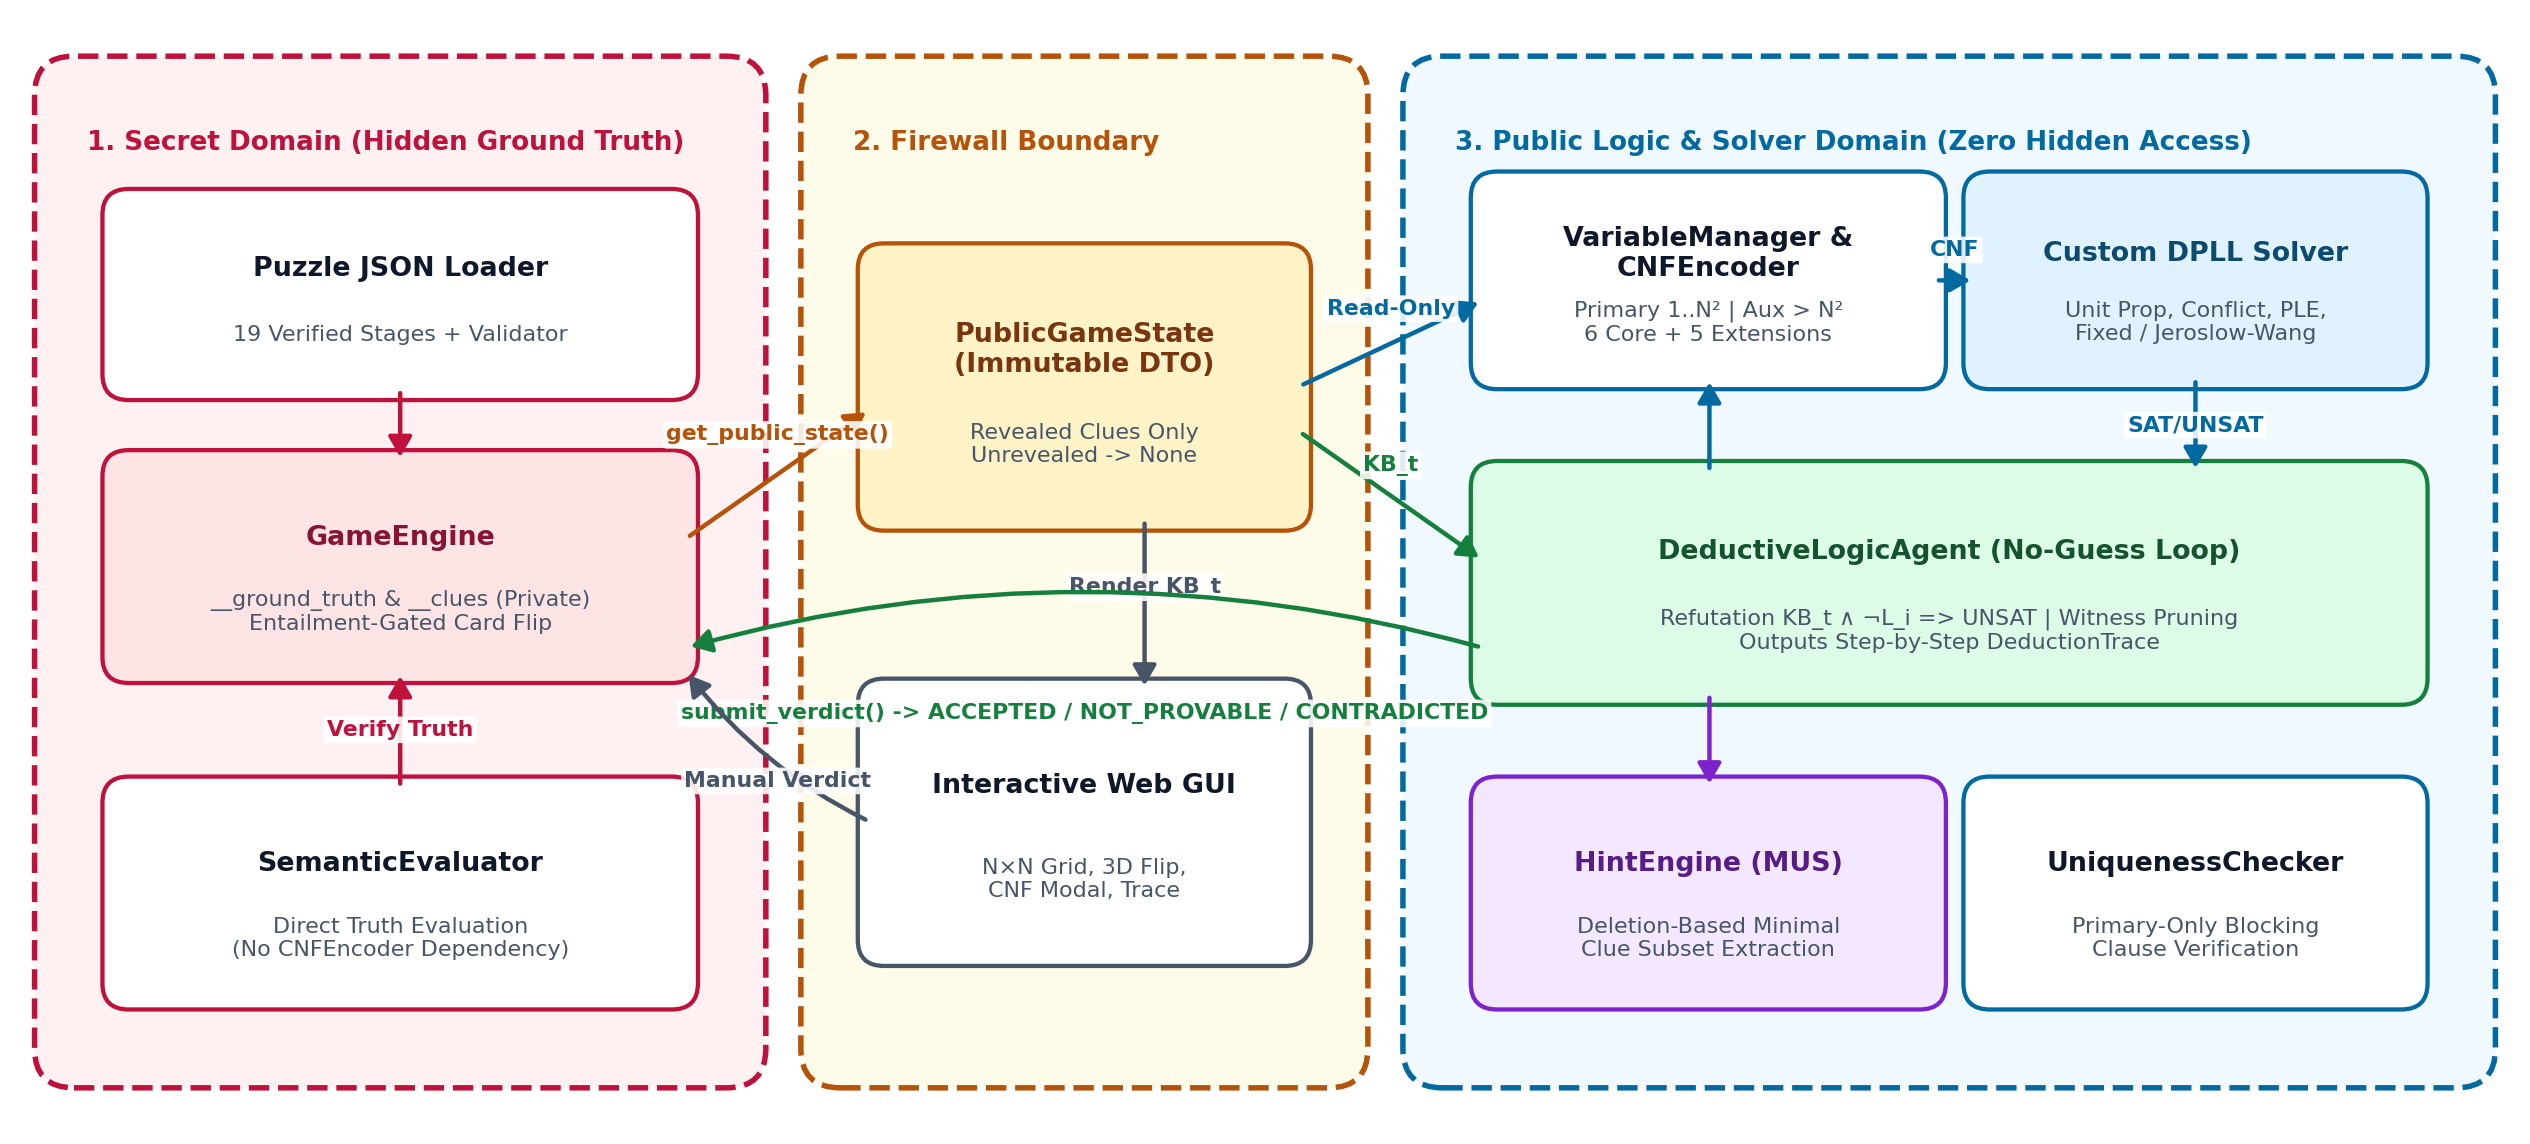
\includegraphics[width=0.96\textwidth]{figures/architecture_diagram.png}
\caption{Three-domain security architecture isolating \texttt{GameEngine} secrets from \texttt{DeductiveLogicAgent}.}
\end{figure}

\section{CNF Encoding Derivations}

\subsection{Binary Clues (\texttt{SAME} and \texttt{DIFFERENT})}
\begin{align*}
\texttt{SAME}(i, j):\quad C_i \leftrightarrow C_j &\equiv (C_i \to C_j) \land (C_j \to C_i) \equiv (\neg C_i \lor C_j) \land (C_i \lor \neg C_j), \\
\texttt{DIFFERENT}(i, j):\quad C_i \oplus C_j &\equiv (C_i \land \neg C_j) \lor (\neg C_i \land C_j) \equiv (C_i \lor C_j) \land (\neg C_i \lor \neg C_j).
\end{align*}
Both encodings produce exactly 2 binary clauses and 0 auxiliary variables.

\subsection{Counting Clues: Combinatorial vs.\ Sinz Sequential Counter}
\paragraph{Direct Combinatorial Derivation for \texttt{EXACTLY(2, \{1, 2, 3, 4\})}:}
Decomposing $\sum_{i=1}^4 \llbracket C_i \rrbracket = 2$ into $\texttt{AT\_MOST}(2, R) \land \texttt{AT\_LEAST}(2, R)$:
\begin{itemize}[nosep]
    \item $\texttt{AT\_MOST}(k, R)$ forbids every $(k+1)$-subset from being all True ($\binom{4}{3} = 4$ clauses):
    \[
    (\neg C_1 \lor \neg C_2 \lor \neg C_3) \land (\neg C_1 \lor \neg C_2 \lor \neg C_4) \land (\neg C_1 \lor \neg C_3 \lor \neg C_4) \land (\neg C_2 \lor \neg C_3 \lor \neg C_4).
    \]
    \item $\texttt{AT\_LEAST}(k, R)$ requires every $(|R|-k+1)$-subset to contain at least one True variable ($\binom{4}{3} = 4$ clauses):
    \[
    (C_1 \lor C_2 \lor C_3) \land (C_1 \lor C_2 \lor C_4) \land (C_1 \lor C_3 \lor C_4) \land (C_2 \lor C_3 \lor C_4).
    \]
\end{itemize}

\paragraph{Sinz (2005) Sequential Counter Derivation for \texttt{AT\_MOST($k$, $[l_1, \dots, l_n]$)}:}
For $1 \le k < n$, allocate $(n-1)k$ auxiliary variables $s_{i,j}$ ($1 \le i \le n-1, 1 \le j \le k$) representing $\sum_{r=1}^i \llbracket l_r \rrbracket \ge j$:
\begin{align*}
i = 1: &\quad (\neg l_1 \lor s_{1,1}) \;\land\; \bigwedge_{j=2}^k (\neg s_{1,j}), \\
2 \le i \le n-1: &\quad (\neg l_i \lor s_{i,1}) \land (\neg s_{i-1,1} \lor s_{i,1}) \land (\neg l_i \lor \neg s_{i-1,k}) \land \bigwedge_{j=2}^k \big[(\neg l_i \lor \neg s_{i-1,j-1} \lor s_{i,j}) \land (\neg s_{i-1,j} \lor s_{i,j})\big], \\
i = n: &\quad (\neg l_n \lor \neg s_{n-1,k}).
\end{align*}
For example, $\texttt{AT\_MOST}(1, \{C_1, C_2, C_3\})$ introduces $s_1, s_2$ and 5 clauses: $(\neg C_1 \lor s_1) \land (\neg C_2 \lor s_2) \land (\neg s_1 \lor s_2) \land (\neg C_2 \lor \neg s_1) \land (\neg C_3 \lor \neg s_2)$.

\subsection{Derivations for Extensions 2, 3, 4, and 5}
\begin{enumerate}[nosep]
    \item \textbf{Regional Count Comparison (\texttt{MORE\_CRIMINALS}):} Canceling $R_1 \cap R_2$, let $R_1' = R_1 \setminus R_2$ and $R_2' = R_2 \setminus R_1$. Introducing $A_j \leftrightarrow \neg C_j$ via $(\neg A_j \lor \neg C_j) \land (A_j \lor C_j)$ for $j \in R_2'$ reduces $\sum_{R_1'} C_i > \sum_{R_2'} C_j$ to $\sum_{i \in R_1'} C_i + \sum_{j \in R_2'} A_j \ge |R_2'| + 1$.
    \item \textbf{Parity Chains (\texttt{PARITY}):} Chaining Tseitin variables $z_m \leftrightarrow (z_{m-1} \oplus l_m)$ via $(\neg z_{m-1} \lor \neg l_m \lor \neg z_m) \land (\neg z_{m-1} \lor l_m \lor z_m) \land (z_{m-1} \lor \neg l_m \lor z_m) \land (z_{m-1} \lor l_m \lor \neg z_m)$ requires $4(|R|-2)+2$ short clauses rather than $2^{|R|-1}$ exponential clauses.
    \item \textbf{Compound Clues (\texttt{COMPOUND}):} Given equisatisfiable CNFs $\exists A_1 F_1(X, A_1)$ and $\exists A_2 F_2(X, A_2)$, disjunction $F_1 \lor F_2$ is encoded via positive selector variables $s_1, s_2$:
    \[
    (s_1 \lor s_2) \;\land\; \bigwedge_{D \in F_1} (\neg s_1 \lor D) \;\land\; \bigwedge_{E \in F_2} (\neg s_2 \lor E).
    \]
    Since existential quantification distributes over disjunction, setting $s_b = \text{False}$ satisfies all relaxed clauses $(\neg s_b \lor \cdot)$ trivially without constraining $A_b$. Implication $\Phi_1 \to \Phi_2$ reduces via structural De Morgan negation to $\text{OR}(\neg \Phi_1, \Phi_2)$.
    \item \textbf{Orthogonal Connectivity (\texttt{CONNECTED}):} On 1D contiguous chains $l_1, \dots, l_m$, connectivity is equivalent to forbidding $(1 \dots 0 \dots 1)$ triples: $\bigwedge_{1 \le a < b < c \le m} (\neg l_a \lor l_b \lor \neg l_c)$ (0 aux vars). On general 2D regions $G_R = (R, E_R)$ with $|R|=m$, we elect a unique minimum-index active root $r_i \leftrightarrow (l_i \land \bigwedge_{p < i} \neg l_p)$ and propagate $(m-1)$ BFS layers $d_{i,t}$ ($d_{i,0} = r_i$):
    \[
    \bigwedge_{t=1}^{m-1} \bigwedge_{i=1}^m \Big[(\neg d_{i,t} \lor l_i) \land \big(\neg d_{i,t} \lor d_{i,t-1} \lor \bigvee_{j \in N_R(i)} d_{j,t-1}\big)\Big] \;\land\; \bigwedge_{i=1}^m (\neg l_i \lor d_{i,m-1}).
    \]
\end{enumerate}

\section{Algorithms, Formal Proofs, and Worked Trace}

\subsection{Formal Correctness Theorems}

\begin{theorem}[Soundness \& Completeness of Witness-Guided Refutation Pruning]
Suppose $KB_t$ is satisfiable with baseline model $M_0 \models KB_t$. Let $\mathcal{W} \supseteq \{M_0\}$ be the set of satisfying models of $KB_t$ observed up to cell $i$. Witness-Guided Pruning classifies cell $i$ identically to full two-query refutation ($KB_t \land \neg C_i$ and $KB_t \land C_i$).
\end{theorem}
\begin{proof}
Because $M_0 \in \mathcal{W}$ assigns every primary variable $C_i$ either True or False, at least one polarity of $C_i$ already has a concrete model $M \in \mathcal{W}$ satisfying $KB_t$. (Case 1) If $\exists M^+, M^- \in \mathcal{W}$ with $M^+(C_i)=\text{True}$ and $M^-(C_i)=\text{False}$, then both $KB_t \land C_i$ and $KB_t \land \neg C_i$ are satisfiable, so $i$ is \texttt{UNKNOWN} with zero extra SAT calls. (Case 2) If all $M \in \mathcal{W}$ satisfy $M(C_i) = \text{True}$, then $KB_t \land C_i$ is already satisfiable; testing only $KB_t \land \neg C_i$ yields \texttt{UNSAT} iff $KB_t \models C_i$ (\texttt{CRIMINAL}), and otherwise returns a witness $M^-$ proving \texttt{UNKNOWN}. The case $M(C_i) = \text{False}$ is symmetric.
\end{proof}

\begin{theorem}[Primary-Only Blocking Clause Uniqueness]
Let $KB_{\text{full}}(C, A)$ be an equisatisfiable CNF over primary variables $C = (C_1, \dots, C_{N^2})$ and auxiliary variables $A$, with $M^* \models KB_{\text{full}}$. Then $KB_{\text{full}} \land \bigvee_{i=1}^{N^2} (\neg C_i \text{ if } M^*(C_i) \text{ else } C_i)$ is UNSAT iff $M^*|_C$ is the unique valid Criminal/Innocent assignment of the puzzle.
\end{theorem}
\begin{proof}
Any assignment $(C', A') \models KB_{\text{full}}$ satisfies the primary blocking clause iff $\exists i \in \{1,\dots,N^2\}$ such that $C'_i \neq M^*(C_i)$, i.e., $C' \neq M^*|_C$. Because $A$ is excluded from the blocking clause, alternate auxiliary witnesses $(M^*|_C, A')$ for the same primary assignment $M^*|_C$ violate the blocking clause and cannot cause false non-uniqueness reports.
\end{proof}

\begin{theorem}[Deletion-Based MUS Hint Minimality]
Given an entailed literal $L_{i^*}$ ($KB_t \land \neg L_{i^*}$ is UNSAT), let $\mathcal{C}^* \subseteq \mathcal{R}_t$ be the subset of revealed clues retained after sequential deletion testing. Then $\mathcal{C}^*$ entails $L_{i^*}$ and is subset-minimal (removing any single clue $c \in \mathcal{C}^*$ makes $(\mathcal{C}^* \setminus \{c\}) \land \neg L_{i^*}$ satisfiable).
\end{theorem}
\begin{proof}
Loop invariant: the working set $\mathcal{C}$ always maintains $\text{CNF}(\mathcal{C}) \land \neg L_{i^*} \equiv \text{UNSAT}$ because a clue $c$ is deleted only when UNSAT holds without $c$. By monotonicity of propositional entailment, if removing $c \in \mathcal{C}^*$ caused $(\mathcal{C}_{\text{at } c} \setminus \{c\}) \land \neg L_{i^*}$ to be SAT with model $M$, then $M$ also satisfies $(\mathcal{C}^* \setminus \{c\}) \land \neg L_{i^*}$ since $\mathcal{C}^* \subseteq \mathcal{C}_{\text{at } c}$. Thus no proper subset of $\mathcal{C}^*$ entails $L_{i^*}$.
\end{proof}

\subsection{Time and Space Complexity Summary}
\begin{table}[h!]
\centering
\small
\begin{tabular}{@{}llll@{}}
\toprule
\textbf{Module / Operation} & \textbf{Time Complexity} & \textbf{Space / Clause Size} & \textbf{Notes ($M = N^2$ cells)} \\
\midrule
\texttt{SemanticEvaluator.evaluate} & $O(|R|)$ & $O(M)$ & Direct count / BFS; zero CNF overhead \\
\texttt{CNFEncoder} (Combinatorial) & $O\big(\binom{|R|}{k+1}\big)$ & $\binom{|R|}{k+1}$ clauses, $0$ aux & $|R| \le 8 \implies \le 70$ clauses/clue \\
\texttt{CNFEncoder} (Sinz Counter) & $O(|R|\cdot k)$ & $O(|R|\cdot k)$ clauses \& aux & Linear scaling for large $|R|$ \\
\texttt{DPLLSolver.solve} & $O(2^V \cdot L)$ worst-case & $O(V + L)$ per depth & $V$: total vars, $L$: total literals \\
Deduction Step (Explicit / Pruned) & $\le 2U$ / $\le U+1$ SAT calls & $O(|KB_t|)$ & $U \le M$ unresolved cells \\
\texttt{HintEngine} (Deletion MUS) & $\le |\mathcal{R}_t| + |\mathcal{P}_t| \le 2M$ SAT calls & $O(|KB_t|)$ & Milliseconds for $M \le 25$ \\
\bottomrule
\end{tabular}
\caption{Asymptotic complexity across solver and agent components.}
\end{table}

\subsection{Worked Step-by-Step Hand Trace on \texttt{3x3\_01\_core\_intro} ($KB_0 \to KB_8$)}
Initially, \texttt{A1 (Abel)} is revealed as \texttt{INNOCENT} ($\neg C_{A1}$) with clue \texttt{EXACTLY(2, Row 1)}. Table \ref{tab:trace} traces all 8 deterministic no-guess steps:

\begin{table}[h!]
\centering
\footnotesize
\begin{tabular}{@{}cllp{5.8cm}p{4.3cm}@{}}
\toprule
\textbf{Step} & \textbf{KB Clauses Added} & \textbf{Proved Verdict} & \textbf{Refutation Proof ($KB_t \land \neg L_i \implies \bot$)} & \textbf{Newly Revealed Clue} \\
\midrule
$t=1$ & $(\neg C_{A1})$, $\sum_{\text{Row }1}=2$ & \texttt{B1 = CRIMINAL} & Assume $\neg C_{B1}$: with $\neg C_{A1}$, $(C_{A1} \lor C_{B1})$ yields $\bot$ in 2 unit propagations. & \texttt{B1}: \texttt{DIFFERENT(B1, A2)} \\
$t=2$ & $(C_{B1})$, $(C_{B1} \oplus C_{A2})$ & \texttt{C1 = CRIMINAL} & Assume $\neg C_{C1}$: with $\neg C_{A1}$, $(C_{A1} \lor C_{C1})$ yields $\bot$. & \texttt{C1}: \texttt{EXACTLY(1, Col C)} \\
$t=3$ & $(C_{C1})$, $\sum_{\text{Col C}}=1$ & \texttt{A2 = INNOCENT} & Assume $C_{A2}$: with $C_{B1}$, $(\neg C_{B1} \lor \neg C_{A2})$ yields $\bot$. & \texttt{A2}: \texttt{EXACTLY(1, Row 2)} \\
$t=4$ & $(\neg C_{A2})$, $\sum_{\text{Row }2}=1$ & \texttt{B2 = CRIMINAL} & Col C$=1$ with $C_{C1}$ forces $\neg C_{C2}$; Row 2$=1$ with $\neg C_{A2}, \neg C_{C2}$ forces $C_{B2}$. & \texttt{B2}: \texttt{AT\_LEAST(3, Nbr(B2))} \\
$t=5$ & $(C_{B2})$, $\sum_{\text{Nbr(B2)}} \ge 3$ & \texttt{C2 = INNOCENT} & Assume $C_{C2}$: with $C_{C1}$, $(\neg C_{C1} \lor \neg C_{C2})$ yields $\bot$. & \texttt{C2}: \texttt{SAME(B2, A3)} \\
$t=6$ & $(\neg C_{C2})$, $(C_{B2} \leftrightarrow C_{A3})$ & \texttt{A3 = CRIMINAL} & Assume $\neg C_{A3}$: with $C_{B2}$, $(\neg C_{B2} \lor C_{A3})$ yields $\bot$. & \texttt{A3}: \texttt{AT\_MOST(1, Row 3)} \\
$t=7$ & $(C_{A3})$, $\sum_{\text{Row }3} \le 1$ & \texttt{B3 = INNOCENT} & Assume $C_{B3}$: with $C_{A3}$, $(\neg C_{A3} \lor \neg C_{B3})$ yields $\bot$. & \texttt{B3}: \texttt{NO(\{B3, C3\})} \\
$t=8$ & $(\neg C_{B3})$, $(\neg C_{B3}) \land (\neg C_{C3})$ & \texttt{C3 = INNOCENT} & Assume $C_{C3}$: contradicts unit $(\neg C_{C3})$ (and Col C$=1$). \textbf{SOLVED!} & \texttt{C3}: \texttt{DIFFERENT(A3, C3)} \\
\bottomrule
\end{tabular}
\caption{Complete step-by-step deduction trace from $KB_0$ to $KB_8$ on \texttt{3x3\_01\_core\_intro}.}
\label{tab:trace}
\end{table}

\begin{figure}[h!]
\centering
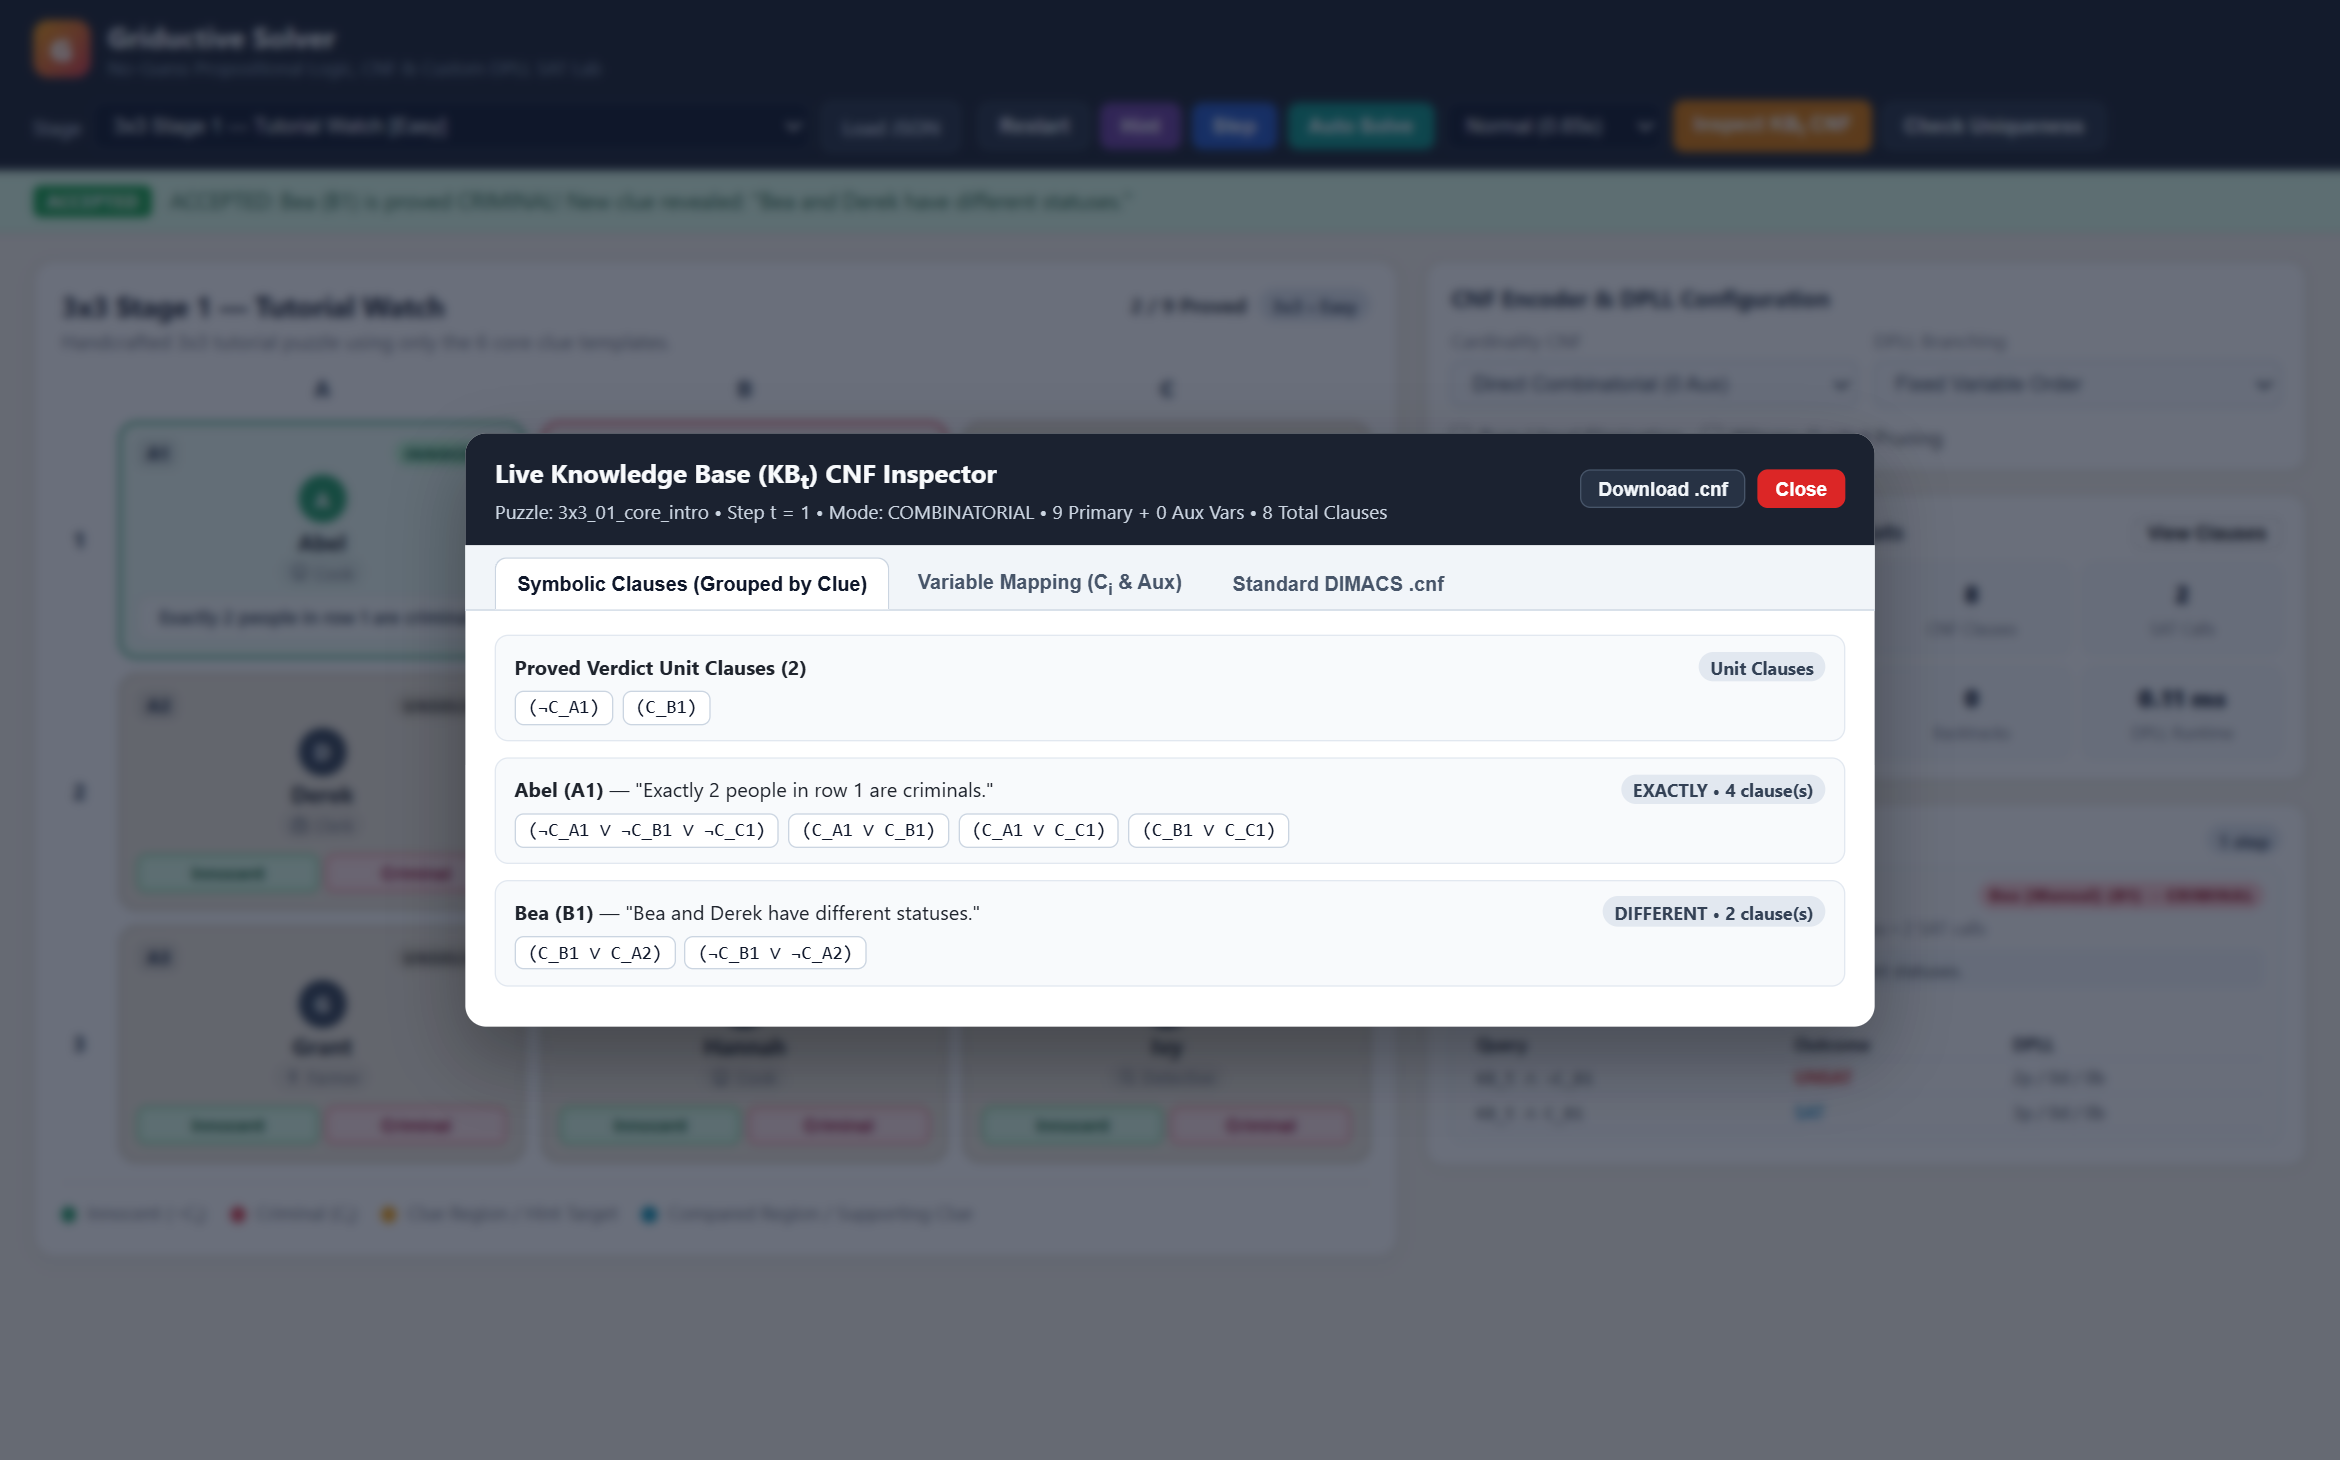
\includegraphics[width=0.90\textwidth]{figures/gui_cnf_inspector.png}
\caption{Live $KB_t$ CNF Inspector Modal showing symbolic clauses grouped by revealed clue, variable map, and DIMACS export.}
\end{figure}

\section{Experimental Evaluation}
All 4 solver/encoding configurations were evaluated on the exact same 19-puzzle suite (6 grids of $3\times 3$ including \texttt{STUCK} and \texttt{INCONSISTENT} cases, 7 grids of $4\times 4$ including 2 coupled backtrack cases, and 6 stress/showcase grids of $5\times 5$). Full figures (\texttt{chart\_sat\_calls\_and\_decisions.png}, \texttt{chart\_backtracks\_coupled.png}, \texttt{chart\_runtime\_by\_grid.png}, \texttt{chart\_clauses\_comb\_vs\_seq.png}) and raw CSV logs are provided in \texttt{Source/experiments/results/}.

\begin{itemize}[nosep]
    \item \textbf{Coupled Backtracking \& Jeroslow-Wang Gain:} Coupled overlapping cardinality and parity puzzles (\texttt{4x4\_06}, \texttt{4x4\_07}, \texttt{5x5\_04}, \texttt{5x5\_05}) contain zero initial unit clauses, causing fixed lexical variable ordering (\texttt{1\_Comb\_Fixed}) to thrash across loosely constrained early-row variables (\textbf{1,251 total backtracks}; 645 on \texttt{5x5\_05}). Weighting short active clauses by $2^{-|C|}$ (\texttt{3\_Comb\_JW}) prioritizes coupled cores and cuts total backtracks by \textbf{78.1\% (1,251 $\to$ 274)} on the exact same 4,370 SAT calls.
    \item \textbf{Witness-Guided Pruning:} \texttt{4\_Comb\_JW\_Pruned} further cuts SAT calls by \textbf{45.5\% (4,370 $\to$ 2,380)}, decisions by \textbf{61.3\% (6,679 $\to$ 2,586)}, and total runtime by \textbf{37.9\% (10.11s $\to$ 6.28s)}.
    \item \textbf{Cardinality Encoding Trade-off:} Because Griductive regions satisfy $|R| \le 8$, Direct Combinatorial encoding avoids exponential blowup while sparing $17\times$ auxiliary variable propagation overhead compared to Sinz Sequential Counters ($5.2\times$ faster overall).
\end{itemize}

\section{References and Generative AI Appendix}
\begin{enumerate}[nosep,label={[\arabic*]}]
    \item M. Davis and H. Putnam, ``A computing procedure for quantification theory,'' \emph{JACM}, 7(3):201--215, 1960.
    \item M. Davis, G. Logemann, and D. Loveland, ``A machine program for theorem-proving,'' \emph{CACM}, 5(7):394--397, 1962.
    \item C. Sinz, ``Towards an optimal CNF encoding of Boolean cardinality constraints,'' in \emph{Proc.\ CP 2005}, LNCS 3709, pp.\ 827--831.
    \item R. G. Jeroslow and J. Wang, ``Solving propositional satisfiability problems,'' \emph{Ann.\ Math.\ Artif.\ Intell.}, 1:167--187, 1990.
    \item S. Russell and P. Norvig, \emph{Artificial Intelligence: A Modern Approach}, 4th ed., Pearson, 2020, Chapter 7.
    \item Griductive Official Puzzle Game \& Rules: \url{https://griductive.com}.
\end{enumerate}

\paragraph{Appendix — Generative AI Disclosure:} Generative AI tools assisted with roadmap planning, $2^9 = 512$ exhaustive truth-table test generation, UI localization/CSS layout, and report typesetting. Representative prompts included: (1) building a rubric-aligned implementation roadmap; (2) verifying Combinatorial, Sinz Sequential Counter, Tseitin XOR, Compound selector, and 2D BFS Connectivity CNF encodings against a standalone semantic evaluator; and (3) designing coupled non-unit puzzles to stress-test DPLL backtracking heuristics.

\end{document}
